% ACL-style main figure (full text width, 16.0 cm; use \begin{figure*} ... 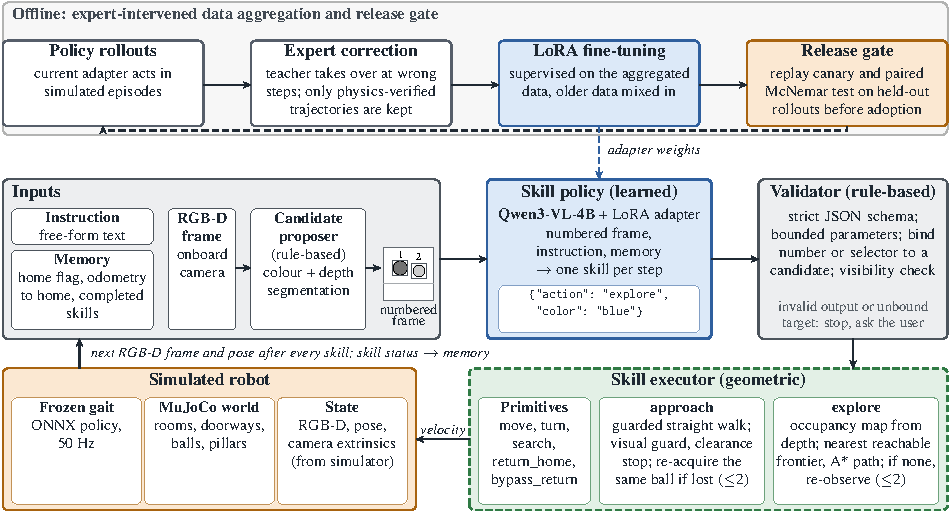
\includegraphics[width=\textwidth]{architecture_acl.pdf})
% Build: cd assets/paper && pdflatex architecture_acl.tex
% Conventions (ACL style files / ACLPUB): Times text, caption set in the paper (not here), vector PDF with embedded fonts,
% readable in grayscale: every module is named and tagged (learned / rule-based / geometric / simulation); colour is never the only cue.
\documentclass[tikz,border=1pt]{standalone}
\usepackage[T1]{fontenc}
\usepackage{times}
\usepackage[scaled=0.92]{inconsolata}
\usetikzlibrary{arrows.meta,calc}

\definecolor{learnedF}{HTML}{DCE9F8} \definecolor{learnedE}{HTML}{2F5F9E}
\definecolor{ruleF}{HTML}{EDEEF0}    \definecolor{ruleE}{HTML}{565E6A}
\definecolor{geoF}{HTML}{E3F0E6}     \definecolor{geoE}{HTML}{2F7A44}
\definecolor{simF}{HTML}{FBE8D2}     \definecolor{simE}{HTML}{A8630F}
\definecolor{ink}{HTML}{1F2933}

\newcommand{\ttl}{\fontsize{8.5}{9.5}\selectfont\bfseries}   % module title
\newcommand{\bdy}{\fontsize{7.5}{8.7}\selectfont}             % module body
\newcommand{\sml}{\fontsize{7}{8}\selectfont}                 % annotations

\tikzset{
  box/.style={rounded corners=2.5pt, line width=0.6pt, draw=ink!80},
  tag/.style={anchor=north, align=center, inner sep=0pt, text=ink, font=\bdy},
  arr/.style={-{Stealth[length=3.6pt,width=3pt]}, line width=0.7pt, draw=ink},
  darr/.style={-{Stealth[length=3.6pt,width=3pt]}, line width=0.7pt, draw=ink, dash pattern=on 3pt off 2pt},
  note/.style={inner sep=1pt, text=ink, font=\sml\itshape},
}

\begin{document}
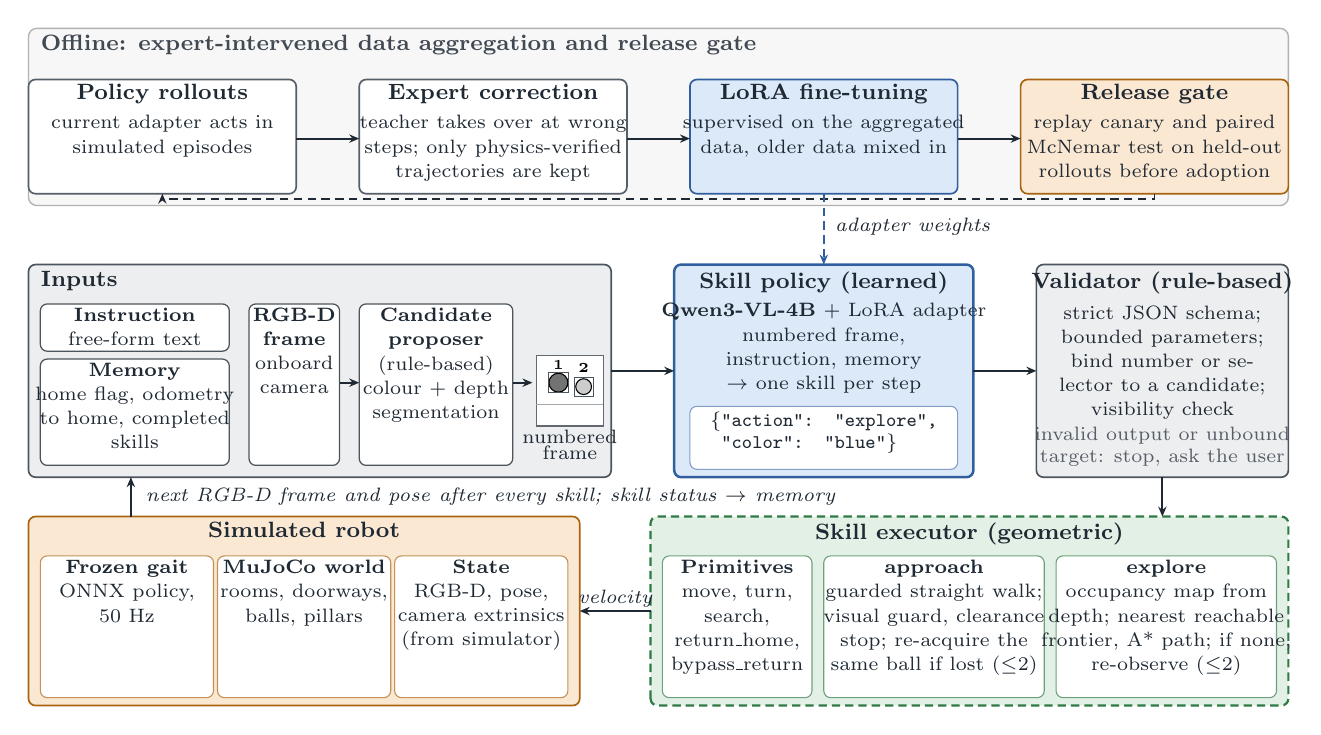
\begin{tikzpicture}[x=1cm,y=1cm]

%%%%%%%%%%%%%%%%%%%%%%%%%%%% offline panel (top)
\draw[rounded corners=3pt, line width=0.5pt, draw=black!30, fill=black!3] (0,6.35) rectangle (16,8.6);
\node[anchor=north west, font=\fontsize{8}{9}\selectfont\bfseries, text=ink!85, inner sep=0pt] at (0.15,8.52)
  {Offline: expert-intervened data aggregation and release gate};

\foreach \x/\t/\d/\f/\e in {
   0/Policy rollouts/{current adapter acts in\\ simulated episodes}/white/ruleE,
   4.2/Expert correction/{teacher takes over at wrong\\ steps; only physics-verified\\ trajectories are kept}/white/ruleE,
   8.4/LoRA fine-tuning/{supervised on the aggregated\\ data, older data mixed in}/learnedF/learnedE,
   12.6/Release gate/{replay canary and paired\\ McNemar test on held-out\\ rollouts before adoption}/simF/simE} {
  \draw[box, draw=\e, fill=\f] (\x,6.5) rectangle (\x+3.4,7.95);
  \node[tag] at (\x+1.7,7.9) {\ttl \t};
  \node[tag] at (\x+1.7,7.5) {\bdy \d};
}
\foreach \a/\b in {3.4/4.2, 7.6/8.4, 11.8/12.6} { \draw[arr] (\a,7.2) -- (\b,7.2); }
\draw[darr] (14.3,6.5) -- (14.3,6.43) -- (1.7,6.43) -- (1.7,6.5);   % next round (kept inside the panel)

%%%%%%%%%%%%%%%%%%%%%%%%%%%% row 1: inputs -> policy -> validator
% inputs (instruction, memory, frame -> candidate proposer -> numbered frame)
\draw[box, fill=ruleF] (0,2.9) rectangle (7.4,5.6);
\node[tag, anchor=north west, inner sep=0pt] at (0.15,5.52) {\ttl Inputs};
\draw[box, line width=0.45pt, fill=white] (0.15,4.5) rectangle (2.55,5.1);
\node[tag] at (1.35,5.06) {\bdy \textbf{Instruction}\\ free-form text};
\draw[box, line width=0.45pt, fill=white] (0.15,3.05) rectangle (2.55,4.4);
\node[tag] at (1.35,4.36) {\bdy \textbf{Memory}\\ home flag, odometry\\ to home, completed\\ skills};
\draw[box, line width=0.45pt, fill=white] (2.8,3.05) rectangle (3.95,5.1);
\node[tag] at (3.375,5.05) {\bdy \textbf{RGB-D}\\ \textbf{frame}\\ onboard\\ camera};
\draw[box, line width=0.45pt, fill=white] (4.2,3.05) rectangle (6.15,5.1);
\node[tag] at (5.175,5.05) {\bdy \textbf{Candidate}\\ \textbf{proposer}\\ (rule-based)\\ colour + depth\\ segmentation};
\draw[arr] (3.95,4.1) -- (4.2,4.1);
\draw[arr] (6.15,4.1) -- (6.4,4.1);
% numbered frame icon
\begin{scope}[shift={(6.45,3.55)}]
  \draw[line width=0.45pt, fill=white, draw=ink!70] (0,0) rectangle (0.85,0.9);
  \draw[line width=0.3pt, draw=ink!40] (0,0.28) -- (0.85,0.28);
  \draw[line width=0.4pt, fill=black!55] (0.28,0.55) circle (0.12);
  \draw[line width=0.4pt, draw=ink!80] (0.15,0.42) rectangle (0.41,0.68);
  \draw[line width=0.4pt, fill=black!20] (0.6,0.5) circle (0.1);
  \draw[line width=0.4pt, draw=ink!80] (0.48,0.38) rectangle (0.72,0.62);
  \node[font=\fontsize{5}{6}\selectfont\bfseries, inner sep=0.2pt, fill=white] at (0.28,0.78) {1};
  \node[font=\fontsize{5}{6}\selectfont\bfseries, inner sep=0.2pt, fill=white] at (0.6,0.74) {2};
\end{scope}
\node[tag] at (6.875,3.5) {\sml numbered};
\node[tag] at (6.875,3.3) {\sml frame};

% skill policy (learned)
\draw[box, line width=0.9pt, draw=learnedE, fill=learnedF] (8.2,2.9) rectangle (12.0,5.6);
\node[tag] at (10.1,5.52) {\ttl Skill policy (learned)};
\node[tag] at (10.1,5.12) {\bdy \textbf{Qwen3-VL-4B} + LoRA adapter};
\node[tag] at (10.1,4.8) {\bdy numbered frame,\\ instruction, memory\\ $\rightarrow$ one skill per step};
\draw[box, line width=0.4pt, draw=learnedE!60, fill=white] (8.4,3.0) rectangle (11.8,3.8);
\node[tag, anchor=north, align=left, inner sep=0pt, font=\fontsize{7}{8}\selectfont\ttfamily] at (10.1,3.74) {\{"action": "explore",\\ \phantom{\{}"color": "blue"\}};

% validator (rule-based)
\draw[box, fill=ruleF] (12.8,2.9) rectangle (16,5.6);
\node[tag] at (14.4,5.52) {\ttl Validator (rule-based)};
\node[tag, text width=2.85cm] at (14.4,5.08) {\bdy strict JSON schema; bounded parameters; bind number or selector to a candidate; visibility check};
\node[tag, text=ink!75, font=\sml] at (14.4,3.55) {invalid output or unbound\\ target: stop, ask the user};

%%%%%%%%%%%%%%%%%%%%%%%%%%%% row 2: executor -> simulator
\draw[box, line width=0.8pt, draw=geoE, fill=geoF, dash pattern=on 3pt off 1.8pt] (7.9,0) rectangle (16,2.4);
\node[tag] at (11.95,2.33) {\ttl Skill executor (geometric)};
\foreach \x/\w/\t/\d in {
   8.05/1.9/Primitives/{move, turn,\\ search,\\ return\_home,\\ bypass\_return},
   10.1/2.8/approach/{guarded straight walk;\\ visual guard, clearance\\ stop; re-acquire the\\ same ball if lost ($\le$2)},
   13.05/2.8/explore/{occupancy map from\\ depth; nearest reachable\\ frontier, A* path; if none,\\ re-observe ($\le$2)}} {
  \draw[box, line width=0.4pt, draw=geoE!70, fill=white] (\x,0.1) rectangle (\x+\w,1.9);
  \node[tag] at (\x+\w/2,1.85) {\bdy \textbf{\t}\\ \d};
}

\draw[box, fill=simF, draw=simE] (0,0) rectangle (7,2.4);
\node[tag] at (3.5,2.33) {\ttl Simulated robot};
\foreach \x/\t/\d in {
   0.15/Frozen gait/{ONNX policy,\\ 50 Hz},
   2.4/MuJoCo world/{rooms, doorways,\\ balls, pillars},
   4.65/State/{RGB-D, pose,\\ camera extrinsics\\ (from simulator)}} {
  \draw[box, line width=0.4pt, draw=simE!70, fill=white] (\x,0.1) rectangle (\x+2.2,1.9);
  \node[tag] at (\x+1.1,1.85) {\bdy \textbf{\t}\\ \d};
}

%%%%%%%%%%%%%%%%%%%%%%%%%%%% arrows between rows and rows
\draw[arr] (7.4,4.25) -- (8.2,4.25);
\draw[arr] (12.0,4.25) -- (12.8,4.25);
\draw[arr] (14.4,2.9) -- (14.4,2.4);
\draw[arr] (7.9,1.2) -- (7.0,1.2);
\node[note, anchor=south] at (7.45,1.2) {velocity};
\draw[arr] (1.3,2.4) -- (1.3,2.9);
\node[note, anchor=west] at (1.45,2.65) {next RGB-D frame and pose after every skill; skill status $\rightarrow$ memory};
\draw[darr, draw=learnedE] (10.1,6.5) -- (10.1,5.6);
\node[note, anchor=west] at (10.2,6.08) {adapter weights};

\end{tikzpicture}
\end{document}
